\documentclass[11pt]{article}
\usepackage[margin=1in]{geometry}
\usepackage[T1]{fontenc}
\usepackage{lmodern}
\usepackage{amsmath,amssymb}
\usepackage{graphicx}
\usepackage{booktabs}
\usepackage{caption}
\usepackage{microtype}
\usepackage[hidelinks]{hyperref}
\captionsetup{font=small,labelfont=bf,width=0.95\textwidth}
\graphicspath{{../figs/}}
% let text share a page with a tall figure instead of forcing float-only pages
\renewcommand{\topfraction}{0.95}
\renewcommand{\bottomfraction}{0.6}
\renewcommand{\textfraction}{0.05}
\renewcommand{\floatpagefraction}{0.85}

\newcommand{\eps}{\epsilon}
\newcommand{\sci}[2]{$#1\times10^{#2}$}
\newcommand{\code}[1]{\texttt{#1}}

\title{Computational Physics, Homework 3:\\
Fourier transforms --- sunspot periodicity, Fourier filtering,
and image deconvolution}
\author{Xuanzhe Xia \\ \texttt{xx2720@nyu.edu} \\[4pt]
\small Code: \url{https://github.com/hz-xiaxz/compphys-hw3}}
\date{October 18, 2026}

\begin{document}
\maketitle

\section*{Summary}

This assignment applies the discrete Fourier transform to three data sets from
the online resources of Newman's \emph{Computational Physics}. All transforms
use \code{numpy.fft}.

In the first part (Exercise~7.2) I estimated the length of the solar cycle from
the monthly sunspot record for 1749--2010 in two ways. The 24 maxima of the
smoothed series are on average 130.4 months apart. The power spectrum
$|c_k|^2$ has its largest peak at $k=24$, which corresponds to a period
$N/k = 3143/24 = 131.0$ months, or 10.9 years. The two estimates agree to
0.5 months, far less than the 24-month scatter in the lengths of individual
cycles.

In the second part (Exercise~7.4) I low-pass filtered 1024 daily closing values
of the Dow Jones Industrial Average by zeroing all but the first 10\% (and then
2\%) of the 513 coefficients returned by \code{rfft} and transforming back. Keeping
10\% removes every fluctuation faster than about 20 business days (one month)
and leaves a smooth curve that follows the 2007 peak, the 2008 crash and the
March 2009 low. Keeping 2\% leaves only periods longer than about 114 business
days, so only the overall trend survives. Both filtered curves are pulled
towards the same value at the two ends, because the DFT treats the series as
periodic and the last closing value is 644 points below the first.

In the third part (Exercise~7.9) I deblurred a photograph that had been blurred
with a Gaussian point spread function of width $\sigma=25$ pixels, by dividing
its 2D Fourier transform by that of the point spread function. With the
threshold $\eps=10^{-3}$ suggested in the book, the half-timbered house in the
photo becomes clearly visible. The data are stored to five decimal places, and
this rounding noise is the only noise in them, so the threshold can be pushed
down to $\eps\approx10^{-8}$ before the amplified noise becomes visible, which
gives a noticeably sharper image. Pushing it further, to $10^{-10}$, destroys the
image. This answers part~(d) quantitatively: the Gaussian blur attenuates the
Fourier mode $q$ by $e^{-2\pi^2\sigma^2q^2}$, so modes whose attenuated amplitude
falls below the noise are lost for good. The noise in the output grows as
$1/\eps$, but the resolution improves only as $\sqrt{\ln(1/\eps)}$: going from
$\eps=10^{-3}$ to $10^{-8}$ multiplies the noise by $10^5$ but improves the
resolution only from 42 to 26 pixels.

\section*{Methods}

\subsection*{Discrete Fourier transform conventions}

For $N$ real samples $y_n$, \code{numpy.fft.rfft} returns the
$\tfrac12N+1$ coefficients
\[
c_k = \sum_{n=0}^{N-1} y_n\, e^{-2\pi i kn/N}, \qquad k = 0,\dots,\lfloor N/2\rfloor,
\]
which is Newman's Eq.~(7.15); the remaining coefficients are their complex
conjugates, $c_{N-k}=c_k^*$. \code{irfft} inverts the transform,
$y_n = N^{-1}\sum_{k=0}^{N-1} c_k e^{2\pi ikn/N}$. The term $c_k$ is a wave with
$k$ cycles across the data, i.e., period $N/k$ samples. The 2D versions
\code{rfft2} and \code{irfft2} act on a $K\times L$ array in the same way, along
both axes.

\subsection*{Problem 1: sunspot periodicity (Exercise 7.2)}

\paragraph{(a) Cycle length from the time series.}
The monthly sunspot numbers fluctuate strongly from month to month, so I first
smoothed them with the standard 13-month running mean (equal weights on the
central 11 months, half weights on the two ends) used in solar physics. The
maxima of the smoothed series were located with \code{scipy.signal.find\_peaks},
requiring maxima to be at least 84 months (7 years) apart and to rise at least
40 above the neighbouring minima. If the first and last of $M$ maxima fall in
months $m_1$ and $m_M$, the mean cycle length is $(m_M-m_1)/(M-1)$.

\paragraph{(b, c) Power spectrum.}
I computed $c_k$ for all $N=3143$ months with \code{rfft} and plotted
$|c_k|^2$ against $k$. The $k=0$ term, $c_0 = N\langle y\rangle$, only measures
the mean sunspot number and is left out. The period corresponding to the
largest remaining peak is $N/k$ months. Since the length of the cycle varies,
the peak spreads over several neighbouring $k$; as a second estimate I also
computed the power-weighted mean $k$ over the bins $k=20$--28 that make up the
peak.

\subsection*{Problem 2: Fourier filtering and smoothing (Exercise 7.4)}

The file \code{dow.txt} holds $N=1024$ closing values, so \code{rfft} returns
513 coefficients. Keeping the first 10\% means keeping $k = 0,\dots,50$ (51
coefficients) and setting $k=51,\dots,512$ to zero; keeping 2\% means keeping
$k=0,\dots,9$. The inverse transform \code{irfft} of the truncated array is
then plotted on top of the data.

Zeroing all coefficients above $k_{\mathrm{cut}}$ is an ideal low-pass filter:
it deletes every sinusoidal component with a period shorter than
$N/k_{\mathrm{cut}}$ samples and leaves the rest untouched. In real space it is
a circular convolution of the data with the kernel
$\sin[\pi(2k_{\mathrm{cut}}-1)n/N]/[N\sin(\pi n/N)]$, a weighted running
average whose width is about $N/2k_{\mathrm{cut}}$ samples.

As a check on the end effects discussed in the Results, I also applied the same
filter with the type-II discrete cosine transform (\code{scipy.fft.dct},
orthonormal), keeping the same fraction of its $N$ coefficients (102 and 20).
The DCT implicitly mirrors the series, $y_0,\dots,y_{N-1},y_{N-1},\dots,y_0$,
before making it periodic, so it does not join the last value to the first.

\subsection*{Problem 3: image deconvolution (Exercise 7.9)}

\paragraph{(a) The photo.}
\code{blur.txt} is read with \code{numpy.loadtxt} into a $1024\times1024$ array
and drawn with \code{imshow} in grey scale. With the default
\code{origin="upper"}, row 0 of the file is drawn at the top, and the image
appears the right way up: bright sky at the top, dark ground at the bottom.

\paragraph{(b) The point spread function.}
The Gaussian $f(x,y)=\exp[-(x^2+y^2)/2\sigma^2]$ with $\sigma=25$ is sampled on
an array of the same size as the photo. The point spread function must be
periodic, so pixel $j$ along each axis stands for the displacement
$\min(j, K-j)$; negative displacements wrap round to the far end of the axis,
and a quarter of the Gaussian ends up in each corner of the array. I normalized
$f$ to unit sum (the unnormalized Gaussian sums to $2\pi\sigma^2 = 3927$).
With this normalization the blur conserves the total brightness, the Fourier
transform of $f$ is $\tilde f(0)=1$, and $\tilde f(q)$ is the factor by which
the blur attenuates the Fourier mode with spatial frequency $q$. Numerically
$\tilde f$ is real and equal to $e^{-2\pi^2\sigma^2q^2}$ to machine precision,
where $q = \sqrt{(k/K)^2+(l/L)^2}$ (with $k$ wrapped to $-K/2\le k<K/2$) is in
cycles per pixel.

\paragraph{(c) Deconvolution.}
A periodic blur is a circular convolution,
$b_{mn} = \sum_{m'n'} a_{m'n'} f_{m-m',\,n-n'}$, and the DFT turns it into a
product, $\tilde b_{kl} = \tilde a_{kl}\tilde f_{kl}$. (Newman writes this as
$\tilde b_{kl} = KL\,\tilde a_{kl}\tilde f_{kl}$, because he normalizes the
transform of the continuous functions by $1/KL$; with \code{numpy}'s unnormalized
\code{rfft2} the factor is absent.) The program therefore
(i)~reads the blurred photo, (ii)~builds the point spread function,
(iii)~transforms both with \code{rfft2}, (iv)~divides $\tilde b_{kl}$ by
$\tilde f_{kl}$ wherever $|\tilde f_{kl}| > \eps$ and leaves the other
coefficients unchanged, (v)~transforms back with \code{irfft2}, and (vi)~draws
the result. Because $\tilde f(0)=1$, $\eps$ is a relative threshold: modes that
the blur has attenuated by more than a factor $1/\eps$ are not restored. For a
Gaussian these are all the modes above the cut-off frequency
\[
q_c(\eps) = \frac{\sqrt{\ln(1/\eps)}}{\sqrt2\,\pi\sigma},
\]
and I quote $1/q_c$, the shortest wavelength restored, as the resolution of the
deblurred image. I ran the deconvolution for
$\eps = 10^{-2}, 10^{-3}, 10^{-6}, 10^{-8}, 10^{-9}, 10^{-10}$ and $10^{-12}$.
As a consistency check, each deblurred image was blurred again with the same
point spread function and compared with the data.

\paragraph{(d) Noise.}
The values in \code{blur.txt} are written with five decimal places, so they
carry a rounding error that is uniformly distributed in
$\pm5\times10^{-6}$, with rms $\sigma_{\mathrm{in}} = 10^{-5}/\sqrt{12} =
2.9\times10^{-6}$. To measure how the deconvolution amplifies it, I generated
an array of such rounding errors, put it through exactly the same deconvolution,
and recorded the rms of the output for 23 values of $\eps$ between $10^{-12}$
and $10^{-1}$. I also computed the median of $|\tilde b|$ over rings of
constant $q$, to see where the spectrum of the photo meets the noise floor. A
rounding error of rms $\sigma_{\mathrm{in}}$ in each pixel gives Fourier
coefficients with rms $\sqrt{KL}\,\sigma_{\mathrm{in}} = 2.96\times10^{-3}$.

\section*{Results}

\subsection*{Problem 1: sunspot periodicity}

\begin{figure}[htbp]
\centering
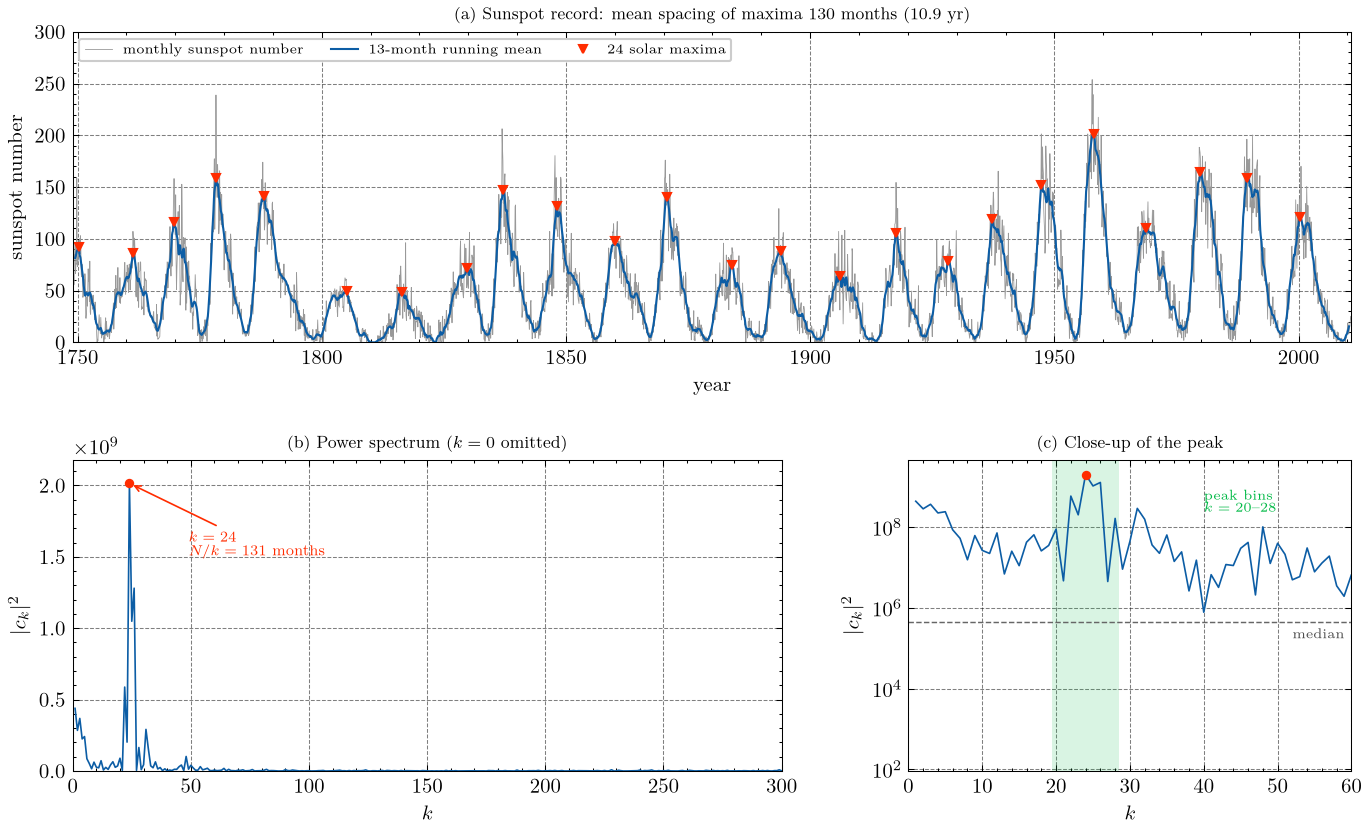
\includegraphics[width=\textwidth]{problem1_sunspots.png}
\caption{Top: monthly sunspot number from January 1749 (grey), its 13-month
running mean (blue), and the 24 maxima found in the running mean (red
triangles). Bottom left: power spectrum $|c_k|^2$ of the sunspot series for
$k\ge1$. Bottom right: the same on a logarithmic scale for $k\le60$; the shaded
band marks the bins $k=20$--28 that make up the peak, and the dashed line is the
median of $|c_k|^2$.}
\label{fig:p1}
\end{figure}

\paragraph{(a)}
The record covers 3143 months, from January 1749 to late 2010 (top panel of
Fig.~\ref{fig:p1}). The sunspot number clearly rises and falls in a regular
cycle over the whole record, although the height of the maxima varies by a
factor of four (it was low around 1800--1820 and highest in the late 1950s).
The smoothed series has 24 maxima, from 1750.2 to 2000.2, so 23 complete cycles
span 250 years. The mean cycle length is therefore
\[
T_a = 130.4\ \text{months} = 10.87\ \text{years}.
\]
Individual cycles range from 88 to 204 months between maxima, with a standard
deviation of 24 months.

\paragraph{(b)}
The power spectrum (bottom left of Fig.~\ref{fig:p1}) has a single dominant peak
at small nonzero $k$, standing far above the low, noisy background. The
largest coefficient after $c_0$ is at $k=24$, followed by $k=26$, 25 and 22;
$|c_{24}|^2$ is about 4600 times the median of $|c_k|^2$.

\paragraph{(c)}
The peak is at $k = 24$, which corresponds to a sine wave with period
\[
T_c = \frac{N}{k} = \frac{3143}{24} = 131.0\ \text{months} = 10.9\ \text{years}.
\]
This agrees with the estimate from part~(a) to 0.5 months (0.4\%). The peak
is several bins wide because the cycle length is not constant: the bins
$k=20$--28 correspond to periods between 112 and 157 months, which is roughly
the spread of individual cycle lengths. The power-weighted mean frequency over
these bins gives a period of 128.4 months. The Fourier estimate is limited by the
bin spacing, $\Delta T \approx T^2/N \approx 5$ months near the peak, so both
Fourier estimates agree with part~(a) within that resolution.

\subsection*{Problem 2: Fourier filtering and smoothing}

\begin{figure}[htbp]
\centering
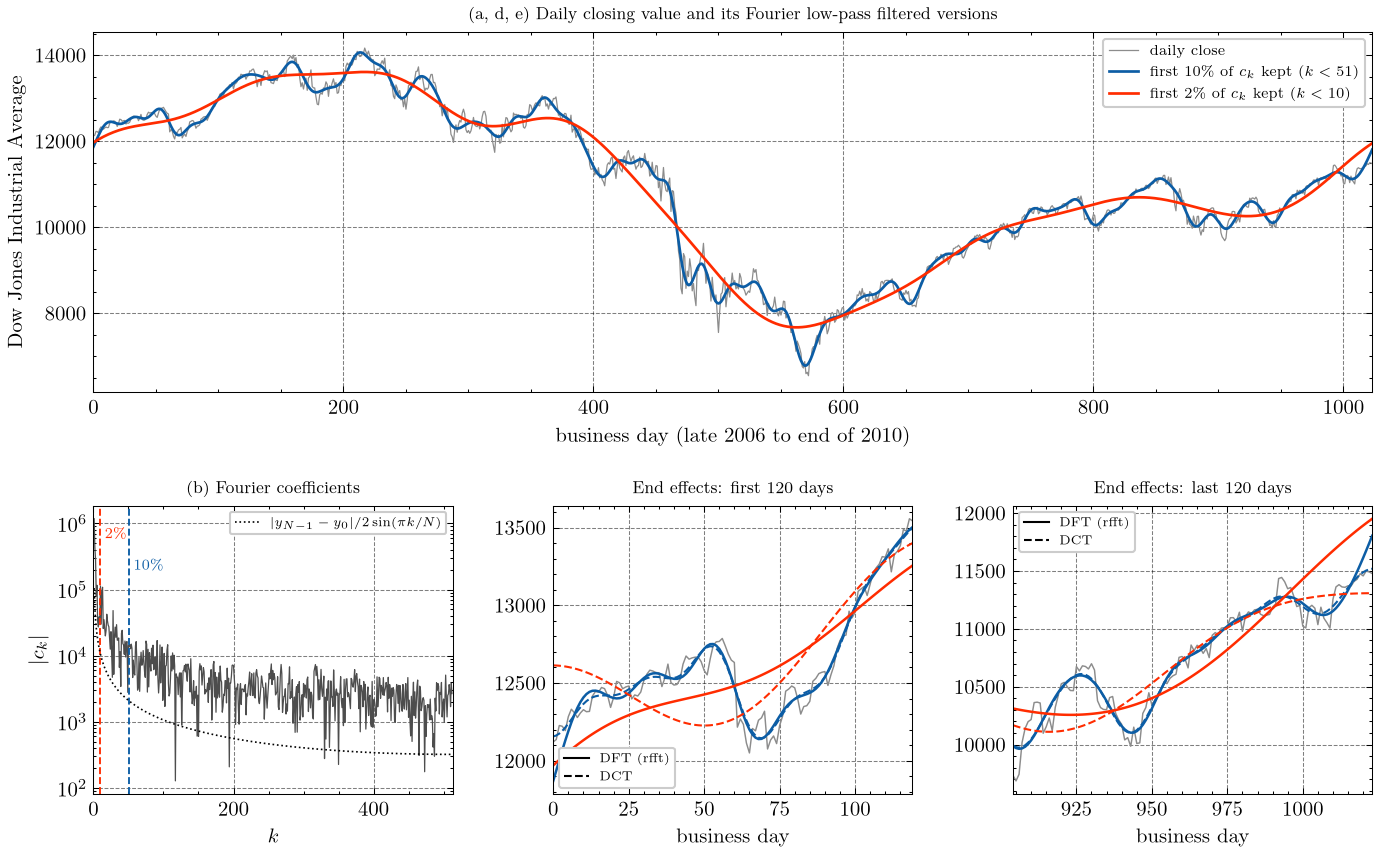
\includegraphics[width=\textwidth]{problem2_dow.png}
\caption{Top: daily closing value of the Dow Jones Industrial Average (grey)
and the inverse transforms after keeping the first 10\% (blue) and 2\% (red) of
the \code{rfft} coefficients. Bottom left: $|c_k|$ with the two cut-offs
(dashed); the dotted line is the contribution expected from the jump between the
last and first values alone. Bottom middle and right: close-ups of the first and
last 120 days, with the DFT-filtered curves (solid) and the same filters applied
with a discrete cosine transform (dashed).}
\label{fig:p2}
\end{figure}

\paragraph{(a, b)}
The 1024 closing values start at 12122 in late 2006, peak at 14165 (day 217,
autumn 2007), fall to 6547 (day 572, March 2009) and recover to 11478 by the
end of 2010 (Fig.~\ref{fig:p2}, top). \code{rfft} returns 513 complex
coefficients. Their magnitude falls steeply over the first few tens of $k$ and
then levels off into a noisy background (bottom left).

\paragraph{(c, d) Keeping 10\%.}
Keeping $k=0,\dots,50$ gives the blue curve. It follows every movement of the
index on time scales of a month or longer --- the 2007 peak, the 2008 crash,
the March 2009 low and the recovery --- but the day-to-day jitter is gone. The
shortest period kept is $N/50 = 20.5$ business days, about one calendar month,
and the rms difference between the data and the smoothed curve is 143 points.
Setting the high-$k$ coefficients to zero removes all the rapidly varying
sinusoids from the Fourier series of the data, so the inverse transform is a
smoothed version of the data. This is a low-pass filter, equivalent to taking
a weighted running average over roughly $N/2k_{\mathrm{cut}}\approx10$ days.
The high-$k$ coefficients are small, so removing 90\% of them changes the curve
only a little.

The filtered curve has one visible defect: near the two ends (bottom panels) it
oscillates and is pulled away from the data. The DFT assumes that the data
repeat with period $N$, so it sees a jump of $-644$ points from the last day
back to the first. That jump needs many high-$k$ components to represent (a
step alone contributes $|c_k|\approx|\Delta|/2\sin(\pi k/N)$, the dotted line
in the bottom-left panel). When they are removed, the filtered curve cannot
follow the jump and smooths it out instead, so both ends are pulled towards the
midpoint 11800: the filtered curve starts at 11871 instead of 12122 and ends
at 11805 instead of 11478, with Gibbs ringing next to them. The DCT does not
have this problem, because the mirrored series has no jump: with the same
fraction of its coefficients the ends are at 12156 and 11519, close to the
data.

\paragraph{(e) Keeping 2\%.}
Keeping only $k=0,\dots,9$ (red curve) leaves only periods longer than
$N/9 = 114$ business days (about 5 months). The result is a smooth curve
that shows only the long-term trend --- a broad rise to the 2007 peak, the fall
to the 2009 low and the recovery --- and misses the shorter rallies and
sell-offs. The rms difference from the data rises to 346 points. The end effect
is even clearer: the curve starts and ends near 11960, much closer together
than the data (12122 and 11478). With so few coefficients, the DCT version has
its own end error, because every cosine has zero slope at the ends, but it is
no longer pulled towards the midpoint.

\subsection*{Problem 3: image deconvolution}

\begin{figure}[htbp]
\centering
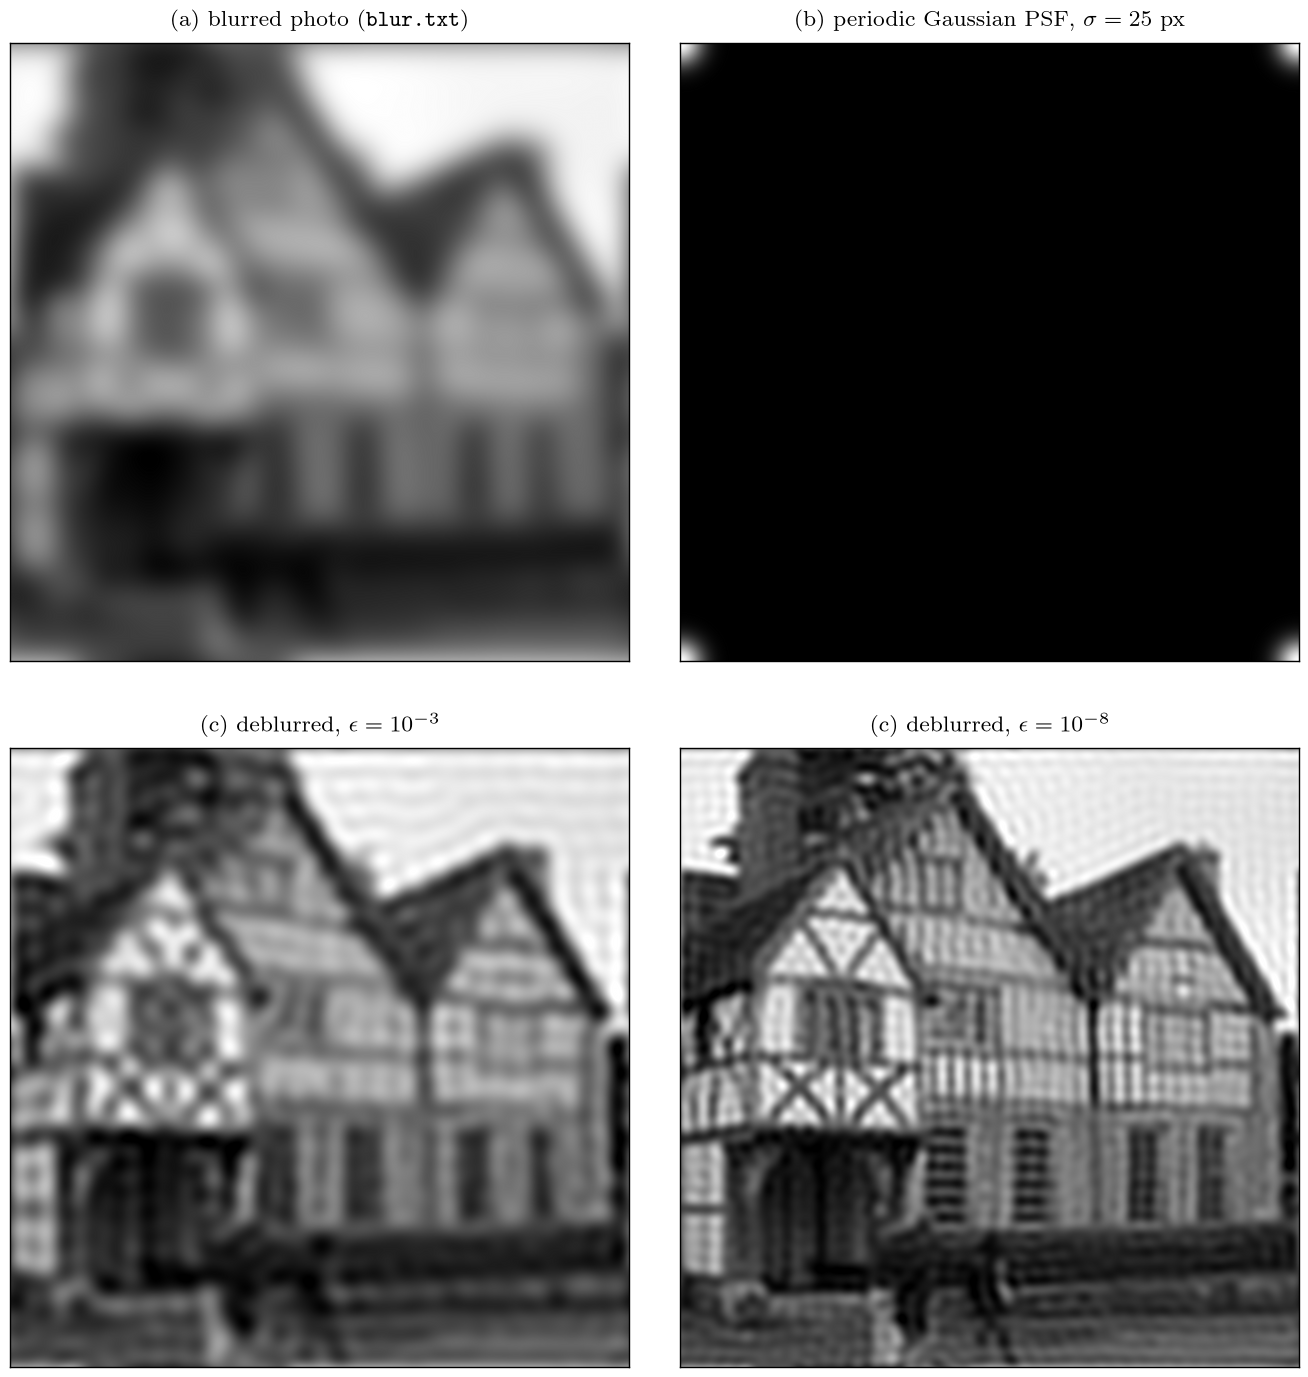
\includegraphics[width=0.86\textwidth]{problem3_deblur.png}
\caption{(a) The blurred photo from \code{blur.txt}. (b) The periodic Gaussian
point spread function, $\sigma=25$ pixels, normalized to unit sum; a quarter of
the Gaussian sits in each corner. (c) The photo deblurred with threshold
$\eps=10^{-3}$ (left) and $\eps=10^{-8}$ (right), shown on the same grey
scale.}
\label{fig:p3}
\end{figure}

\paragraph{(a, b)}
The blurred photo (Fig.~\ref{fig:p3}a) shows only the vague outline of a
building with two gables against a bright sky. Its values range from 101 to 993.
The point spread function (Fig.~\ref{fig:p3}b) has bright quarter-discs in the
four corners, as in the book. The blur has a full width at half maximum of
$2.355\sigma = 59$ pixels.

\paragraph{(c)}
With $\eps = 10^{-3}$, only 0.18\% of the Fourier modes (those with
$q<q_c = 0.024$ cycles per pixel) are divided by $\tilde f$, but that is enough
to reveal a half-timbered house: the diagonal and vertical timbers of the left
gable, the windows, the door, and the roof line of the right-hand house are
all clearly visible (Fig.~\ref{fig:p3}c, left). The image is still soft, and
the hard cut-off in Fourier space adds faint ripples (Gibbs ringing) around
sharp edges, such as the regular pattern in the sky.

Because the only noise in these data is rounding to five decimal places, the
threshold can be lowered much further. Table~\ref{tab:p3} shows the effect.
Each deblurred image, blurred again, reproduces the data to within the rounding
error ($6\times10^{-6}$) once $\eps\le10^{-8}$, which confirms that the
photo was blurred with exactly this periodic Gaussian. With $\eps=10^{-8}$ the
noise in the output is still only 3 brightness units, 0.4\% of the 890-unit
range, and the image is noticeably sharper (Fig.~\ref{fig:p3}c, right, and the
top row of Fig.~\ref{fig:p3lim}): the individual window panes and the timber
crosses are resolved. At $\eps=10^{-9}$ grainy noise starts to
appear, and at $\eps=10^{-10}$ the noise (rms 300) completely buries the
picture. The best threshold for these data is therefore about $10^{-8}$.

\begin{table}[htbp]
\centering
\caption{Deconvolution with different thresholds $\eps$. ``Noise'' is the rms of
the rounding error after it is put through the same deconvolution; ``reblur''
is the largest difference between the data and the deblurred image blurred
again.}
\label{tab:p3}
\begin{tabular}{cccccc}
\toprule
$\eps$ & modes divided & $q_c$ [px$^{-1}$] & $1/q_c$ [px] & noise (rms) & reblur (max) \\
\midrule
$10^{-2}$  & $1.2\times10^{-3}$ & 0.0193 & 52 & $4\times10^{-6}$ & 1.1 \\
$10^{-3}$  & $1.8\times10^{-3}$ & 0.0237 & 42 & $4\times10^{-5}$ & 0.075 \\
$10^{-6}$  & $3.6\times10^{-3}$ & 0.0335 & 30 & 0.034 & $6\times10^{-5}$ \\
$10^{-8}$  & $4.8\times10^{-3}$ & 0.0386 & 26 & 3.2 & $6\times10^{-6}$ \\
$10^{-9}$  & $5.3\times10^{-3}$ & 0.0410 & 24 & 29 & $6\times10^{-6}$ \\
$10^{-10}$ & $5.9\times10^{-3}$ & 0.0432 & 23 & 306 & $6\times10^{-6}$ \\
$10^{-12}$ & $7.1\times10^{-3}$ & 0.0473 & 21 & $3\times10^{4}$ & $6\times10^{-6}$ \\
\bottomrule
\end{tabular}
\end{table}

\begin{figure}[htbp]
\centering
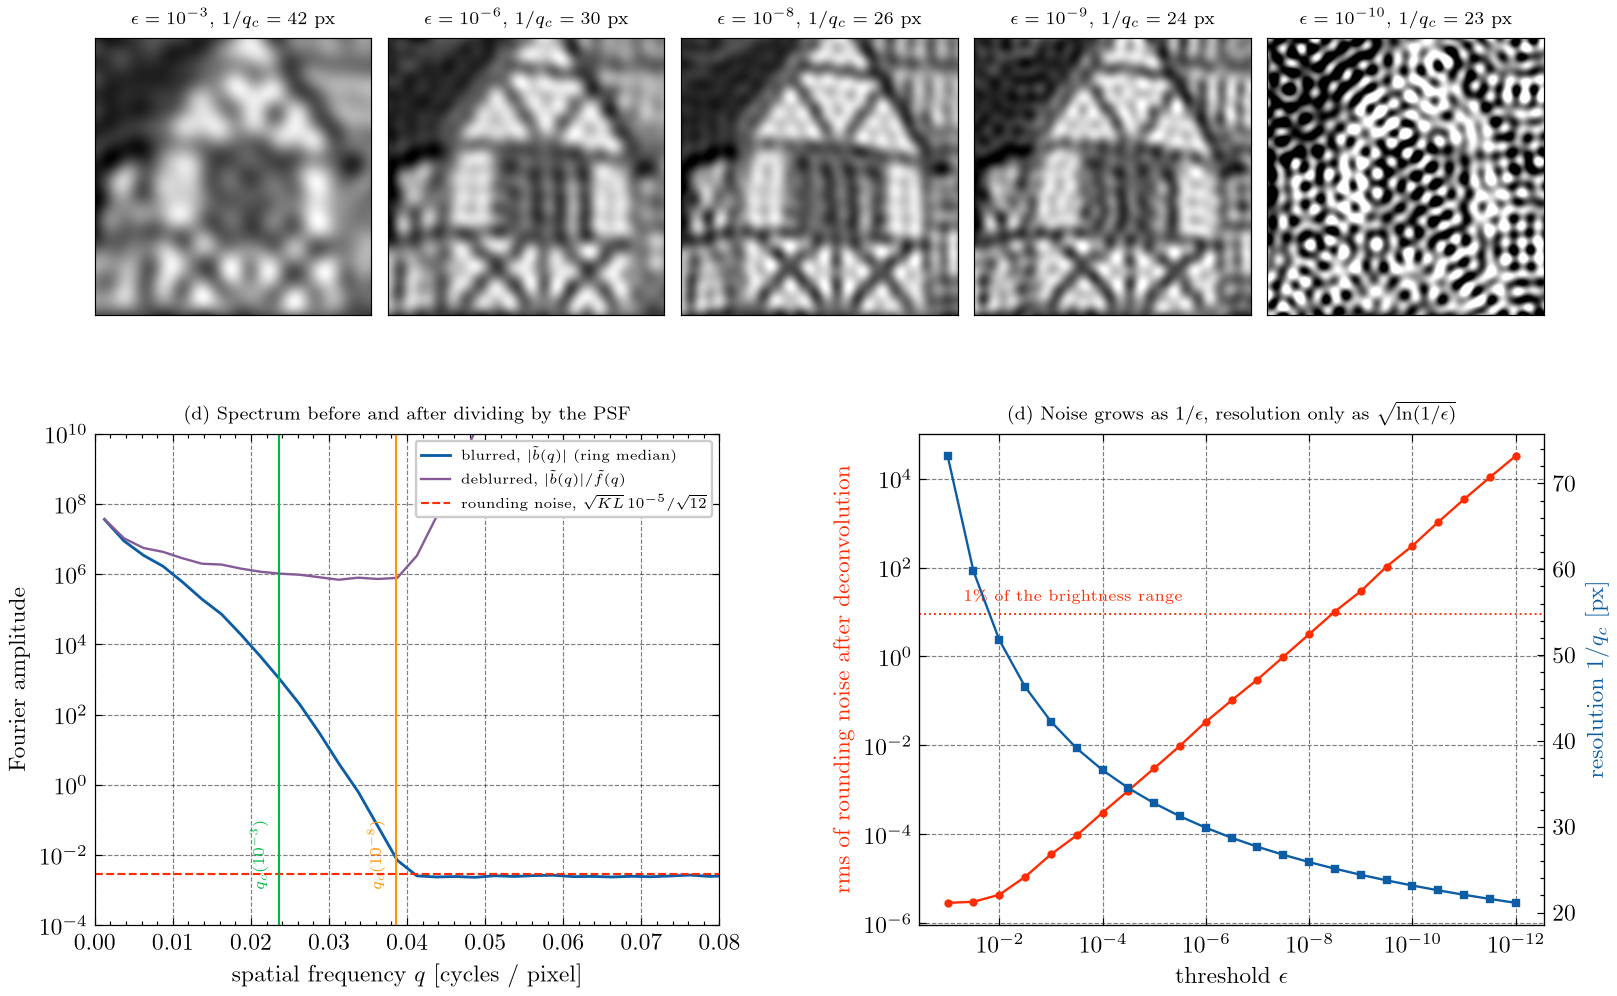
\includegraphics[width=\textwidth]{problem3_limits.png}
\caption{Top: the left gable deblurred with decreasing threshold $\eps$, with
the resolution $1/q_c$ above each panel. Bottom left: median of
$|\tilde b(q)|$ over rings of constant $q$ for the blurred photo (blue) and the
same divided by $\tilde f(q)$ (purple); the dashed line is the expected rms of
the rounding noise, and the vertical lines mark $q_c$ for $\eps=10^{-3}$ and
$10^{-8}$. Bottom right: rms of the rounding noise after deconvolution (red,
left axis) and resolution $1/q_c$ (blue, right axis) as functions of $\eps$;
the dotted line is 1\% of the brightness range of the photo.}
\label{fig:p3lim}
\end{figure}

\paragraph{(d) What limits deblurring?}
The bottom left panel of Fig.~\ref{fig:p3lim} shows what happens. The blur
multiplies the Fourier mode $q$ of the photo by
$\tilde f(q) = e^{-2\pi^2\sigma^2q^2}$, which for $\sigma=25$ is already
$3\times10^{-9}$ at $q=0.04$ and $10^{-54}$ at $q=0.1$. The spectrum of the blurred photo,
$|\tilde b(q)|$, follows this fall until $q\approx0.04$, where it hits a flat
floor at $2.5\times10^{-3}$. That floor is exactly the rounding noise: its
level is $0.83$ times the predicted rms $2.96\times10^{-3}$, and
$\sqrt{\ln2}=0.83$ is the ratio of median to rms for complex Gaussian noise.
Above $q\approx0.04$ the blurred photo contains no information about the
original at all, only noise.

Dividing by $\tilde f$ cannot bring that information back. It amplifies
whatever is in each mode, signal and noise alike, by $1/\tilde f$. Below the
crossing the restored spectrum (purple) is the spectrum of the sharp photo;
above it, it is the noise multiplied by $e^{+2\pi^2\sigma^2q^2}$, which explodes.
This is the same problem the book's hint describes for zeros of $\tilde f$: a
Fourier coefficient of the point spread function that is zero, or so small that
the signal it multiplies is below the noise, destroys that component of the
picture irreversibly. The threshold $\eps$ is just the decision of where to stop
dividing.

The bottom right panel quantifies the trade-off. The output noise grows as
\[
\sigma_{\mathrm{out}} \approx C\,\frac{\sigma_{\mathrm{in}}}{\eps},
\qquad C \approx 0.011,
\]
because the noisiest restored modes are the ones at the cut-off, amplified by
$1/\eps$. The resolution, on the other hand, grows only as
$1/q_c \propto 1/\sqrt{\ln(1/\eps)}$, because $\tilde f$ is a Gaussian: going
from $\eps=10^{-3}$ to $10^{-8}$ multiplies the noise by $10^5$ but improves
the resolution only from 42 to 26 pixels (a factor 1.63). Requiring the
output noise to stay below 1\% of the brightness range gives
$\eps \gtrsim C\sigma_{\mathrm{in}}/(0.01\times\text{range}) = 3.5\times10^{-9}$ for these
data. For an ordinary 8-bit photo, whose rounding error alone is
$\text{range}/(256\sqrt{12})$, the same rule gives $\eps\approx1.2\times10^{-3}$
--- the value the book recommends --- and a resolution of only 43 pixels, still
almost as wide as the blur itself.

So we can never unblur a photo perfectly. In principle a Gaussian blur is
invertible, since $\tilde f$ is never exactly zero, but in practice it suppresses
fine detail far below the level of the noise (from the camera, from photon counting, or at the very least
from storing the brightness with finite precision). Once a Fourier component
has sunk below the noise it is gone, and no amount of computation can recover
it. Lower noise lets us restore more modes, but for a Gaussian blur each extra
factor of ten in signal-to-noise gains less resolution than the previous one.
Even with perfectly known blur the achievable sharpness is set by the noise,
and in real cases the uncertainty in the point spread function itself makes
things worse. Smoother filters (such as the Wiener filter, which weights each
mode by its signal-to-noise ratio instead of cutting off sharply) can reduce
the ringing but cannot get round this limit.

\section*{Code}

All code, the data, the figures and the numerical outputs are in a GitHub
repository:
\begin{center}
\url{https://github.com/hz-xiaxz/compphys-hw3}
\end{center}
The scripts are plain Python (NumPy, SciPy, Matplotlib, SciencePlots) managed
with \code{uv}:
\begin{itemize}
\item \code{problem1.py}: sunspot cycle from the smoothed time series and from
the power spectrum, and \path{figs/problem1_sunspots.png}.
\item \code{problem2.py}: Fourier low-pass filtering of the Dow Jones with 10\%
and 2\% of the coefficients, the DCT comparison, and
\path{figs/problem2_dow.png}.
\item \code{problem3.py}: the periodic Gaussian point spread function, the
deconvolution with a threshold, the noise and resolution analysis, and
\path{figs/problem3_deblur.png} and \path{figs/problem3_limits.png}.
\item \code{plotstyle.py}: shared figure style. \code{data/} holds
\code{sunspots.txt}, \code{dow.txt} and \code{blur.txt} from the book's online
resources, \code{results/} holds the printed output of each script, and
\code{writeup/} holds the source of this document.
\end{itemize}
Running \code{uv sync} followed by \code{uv run python problemN.py} reproduces
every figure and number quoted here.

\end{document}
